\section{Discussion}

% Finding 1: Robustness of few-shot learning methods on biomedical tasks
Our benchmarks reveal that when data is meticulously pre-processed, various few-shot learning algorithms excel in the biomedical field. This outcome is encouraging, showing these methods' robustness in managing the intricate and specialised nature of biomedical data.

% Finding 2: SOT improves meta-learners but not non-meta learners
The most notable finding of our study is the significant role of the SOT module in enhancing the performance of meta-learners in challenging few-shot learning scenarios, as seen on both datasets. This leads to near-perfect generalisation. However, this performance boost is absent in non-meta learners, specifically \texttt{B} and \texttt{B++}. This difference likely stems from their distinct training methods. Meta-learners undergo episodic training that mirrors a few-shot environment with support and query samples across classes. The integration of the transductive SOT feature transform module enables simultaneous optimisation of the main network and the SOT module. This enhances the alignment between support and query samples, crucial for classifying query samples. Conversely, non-meta learners train with random mini-batches and lack a concept of support or query samples. Their inferences are independent, making the SOT's role in facilitating interaction between support and query samples irrelevant. For instance, in Figure~\ref{fig:sot-embeddings}, the SOT embeddings in the \texttt{PN} model demonstrate clear class-based clustering for both support and query samples, a feature not observed in the \texttt{B} model.

% TODO: Adjust title of right subplot
\begin{figure}[h!]
    \centering
    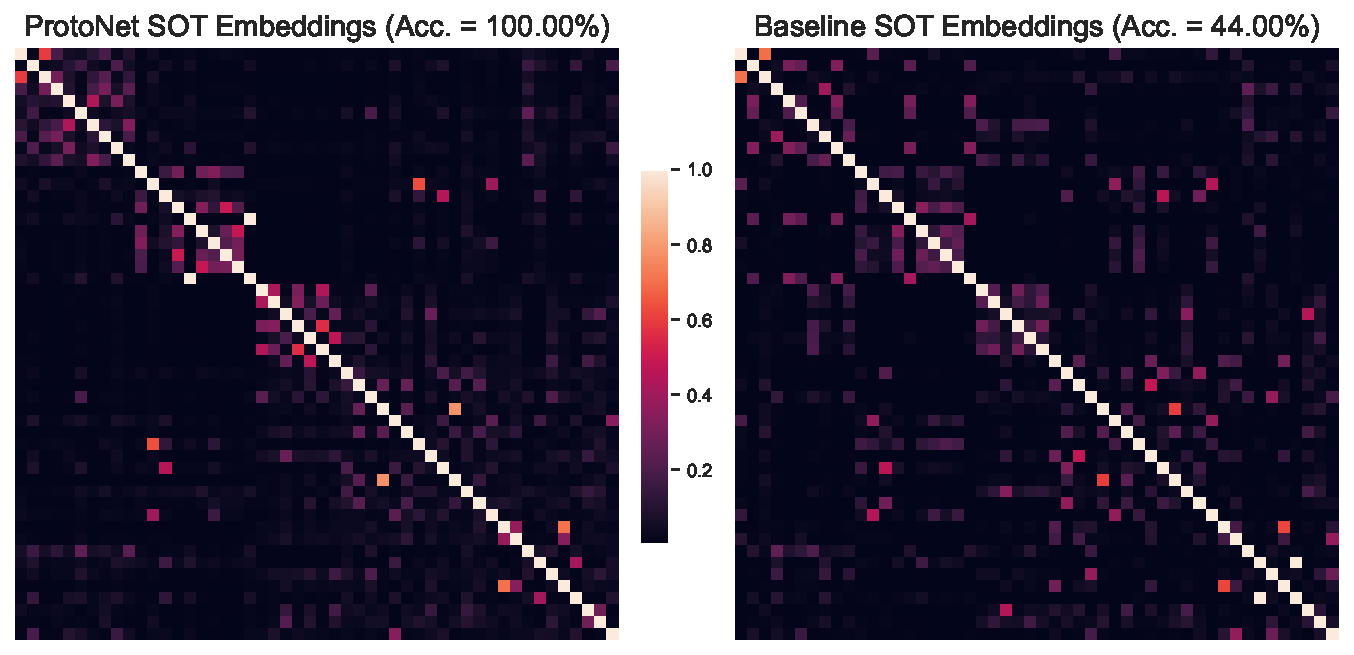
\includegraphics[width=1\columnwidth]{../figures/sot-embeddings.pdf}
    \caption{\textbf{SOT Embeddings.} Heatmap of SOT embeddings for \texttt{PN} (left) and \texttt{B} (right) on the \texttt{SP} dataset for a random test episode in 5-way 5-shot setting. Support and query samples from the same class are adjacent in the embedding matrix.}
    \label{fig:sot-embeddings}
\end{figure}

% Finding 3: SOT improves performance in interaction with LSTM re-embedding
Finally, the ablation study of the re-embedding components in \texttt{MN} suggests that the synergy between the SOT re-embeddings and the LSTM re-embeddings plays a crucial role in the observed performance enhancement of the metric-based meta-learner. The underlying mechanisms of this phenomenon, however, were beyond the purview of this project and are left for future work.
